\section{Antenna and LNA}
Here we  show the  characteristics of  the RF parts.   We show  in the
figure~\ref{fig:vswrant} the VSWR of the antennas. Jacques identified a
bad contact  on the antenna FPV01.   All of the other  antennas have a
low  VSWR (close  to 1  in our
frequency bandwidth as we  expect for  an impedance  match).
\begin{figure}[!ht]
  \centering
  \hspace*{-3ex}
  \subfigure{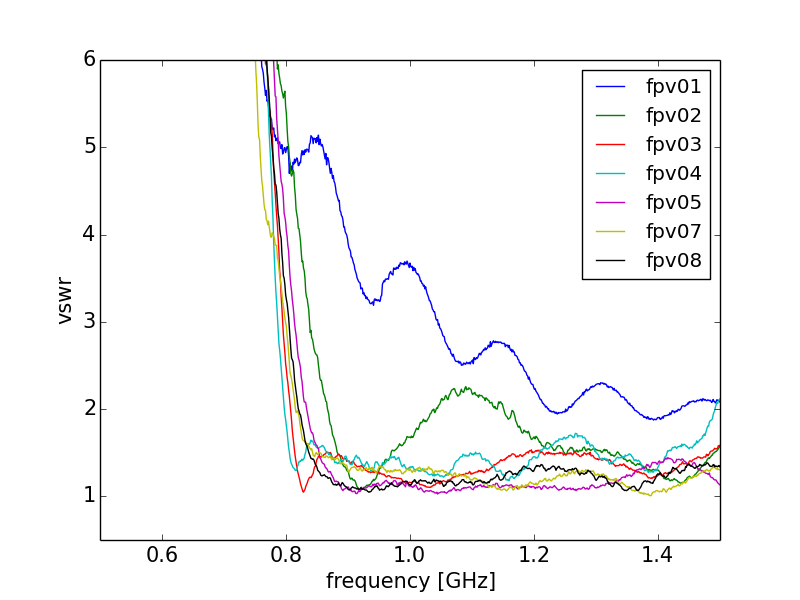
\includegraphics[width=0.60\linewidth]{s11_ant.png}}
  \caption{antenna VSWR, measured in lab}
  \label{fig:vswrant}
\end{figure}

The characteristics  of the LNA were  also measured: the  VSWR and the
gain are shown in the figure~\ref{fig:lnas11} and ~\ref{fig:lnas21}.

\begin{figure}[!ht]
  \centering
  \hspace*{-3ex}
  \subfigure{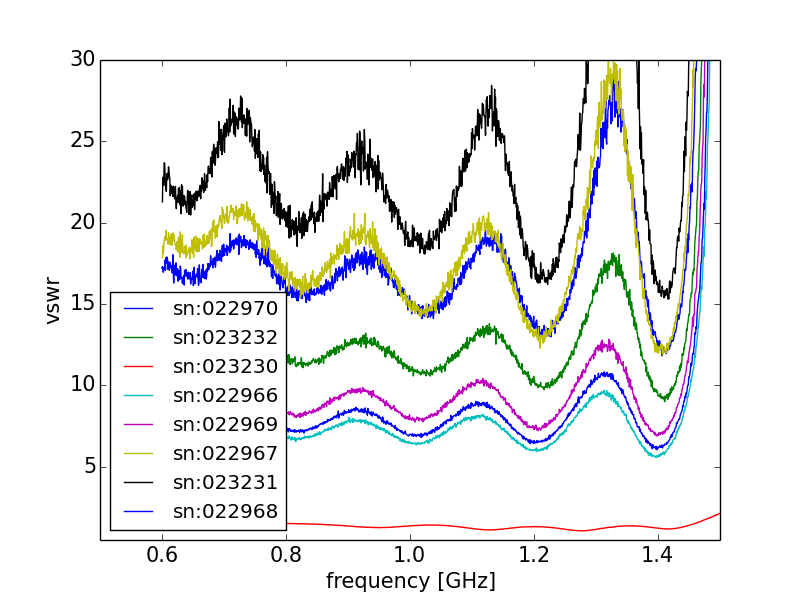
\includegraphics[width=0.60\linewidth]{s11_LNA2.png}}
  \caption{LNA VSWR}
  \label{fig:lnas11}
\end{figure}
\begin{figure}[!ht]
  \centering
  \hspace*{-3ex}
  \subfigure{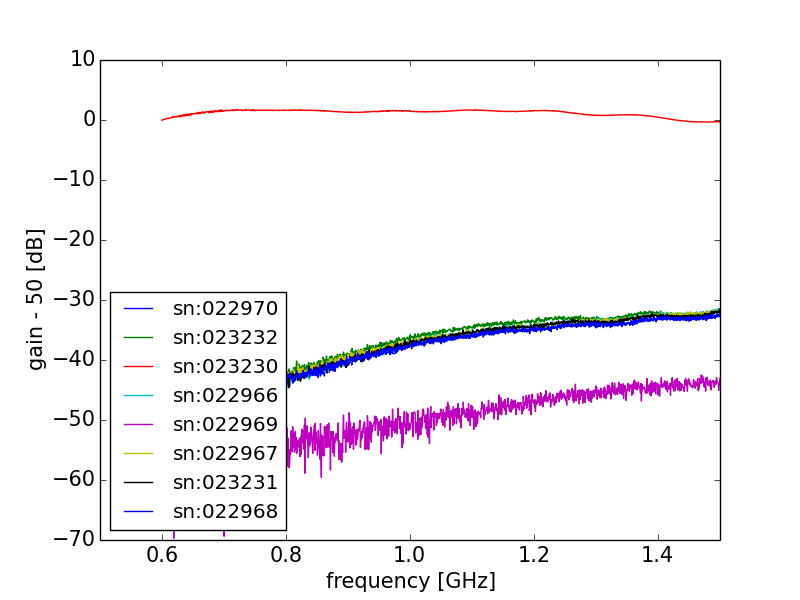
\includegraphics[width=0.60\linewidth]{gain_LNA2.png}}
  \caption{LNA gain. The measurement of the gain was done with a 50dB attenuator.}
  \label{fig:lnas21}
\end{figure}

On the figure \ref{fig:lnas21} it is  clear that only one LNA is still
working, the sn023230, that is the  one that was installed on Nono. It
has the expected gain (50dB) and a low VSWR.  All of the other ones are
broken and almost all have the same characteristics.  \\ So the LNA is
the main failure of the system.  The LNAs broke for an unknown reason.
Possible sources of failure are:
\begin{itemize}
\item a power  surge at the LNA input (for  instance an electro static
  discharge or an over voltage due to a thunderstorm)
\item the humid/water environment (for instance if the LNA was flooded
  inside the box)
\end{itemize}

A  possible  solution  to  the  power  surge could  be  to  install  a
transformer (with coil), or a diode  system before the LNA. We need to
evaluate the effect  of these devices on the  noise figure (since they
need to be placed before the LNA).
